% ========================================
%	Header einbinden
% ========================================

\documentclass[bibtotoc,titlepage]{scrartcl}

% Deutsche Spracheinstellungen
\usepackage[ngerman,german]{babel, varioref}
\usepackage[T1]{fontenc}
\usepackage[utf8]{inputenc}

%\usepackage{marvosym}

\usepackage{amsfonts}
\usepackage{amssymb}
\usepackage{amsmath}
\usepackage{amscd}
\usepackage{amstext}
\usepackage{float}
\usepackage{caption}
\usepackage{wrapfig}
\usepackage{setspace}
\usepackage{threeparttable}
\usepackage{footnote}

\usepackage{caption}
\usepackage{subcaption}

\newfloat{formel}{htbp}{for}
\floatname{formel}{Formel}


\usepackage{longtable}

%\usepackage{bibgerm}

\usepackage{footnpag}

\usepackage{ifthen}                 %%% package for conditionals in TeX
\usepackage{siunitx}
%Fr textumflossene Bilder und Tablellen
%\usepackage{floatflt} - veraltet

%Fr Testzwecke aktivieren, zeigt labels und refs im Text an.
%\usepackage{showkeys}

% Abstand zwischen zwei Abs�zen nach DIN (1,5 Zeilen)
% \setlength{\parskip}{1.5ex plus0.5ex minus0.5ex}

% Einrckung am Anfang eines neuen Absatzes nach DIN (keine)
%\setlength{\parindent}{0pt}

% R�der definieren
% \setlength{\oddsidemargin}{0.3cm}
% \setlength{\textwidth}{15.6cm}

% bessere Bildunterschriften
%\usepackage[center]{caption2}


% Probleml�ungen beim Umgang mit Gleitumgebungen
\usepackage{float}

% Nummeriert bis zur Strukturstufe 3 (also <section>, <subsection> und <subsubsection>)
%\setcounter{secnumdepth}{3}

% Fhrt das Inhaltsverzeichnis bis zur Strukturstufe 3
%\setcounter{tocdepth}{3}

\usepackage{exscale}

\newenvironment{dsm} {\begin{displaymath}} {\end{displaymath}}
\newenvironment{vars} {\begin{center}\scriptsize} {\normalsize \end{center}}


\newcommand {\en} {\varepsilon_0}               % Epsilon-Null aus der Elektrodynamik
\newcommand {\lap} {\; \mathbf{\Delta}}         % Laplace-Operator
\newcommand {\R} { \mathbb{R} }                 % Menge der reellen Zahlen
\newcommand {\e} { \ \mathbf{e} }               % Eulersche Zahl
\renewcommand {\i} { \mathbf{i} }               % komplexe Zahl i
\newcommand {\N} { \mathbb{N} }                 % Menge der nat. Zahlen
\newcommand {\C} { \mathbb{C} }                 % Menge der kompl. Zahlen
\newcommand {\Z} { \mathbb{Z} }                 % Menge der kompl. Zahlen
\newcommand {\limi}[1]{\lim_{#1 \rightarrow \infty}} % Limes unendlich
\newcommand {\sumi}[1]{\sum_{#1=0}^\infty}
\newcommand {\rot} {\; \mathrm{rot} \,}         % Rotation
\newcommand {\grad} {\; \mathrm{grad} \,}       % Gradient
\newcommand {\dive} {\; \mathrm{div} \,}        % Divergenz
\newcommand {\dx} {\; \mathrm{d} }              % Differential d
\newcommand {\cotanh} {\; \mathrm{cotanh} \,}   %Cotangenshyperbolicus
\newcommand {\asinh} {\; \mathrm{areasinh} \,}  %Area-Sinus-Hyp.
\newcommand {\acosh} {\; \mathrm{areacosh} \,}  %Area-Cosinus-H.
\newcommand {\atanh} {\; \mathrm{areatanh} \,}  %Area Tangens-H.
\newcommand {\acoth} {\; \mathrm{areacoth} \,}  % Area-cotangens
\newcommand {\Sp} {\; \mathrm{Sp} \,}
\newcommand {\mbe} {\stackrel{\text{!}}{=}}     %Must Be Equal
\newcommand{\qed} { \hfill $\square$\\}
\renewcommand{\i} {\imath}
\def\captionsngerman{\def\figurename{\textbf{Abb.}}}

%%%%%%%%%%%%%%%%%%%%%%%%%%%%%%%%%%%%%%%%%%%%%%%%%%%%%%%%%%%%%%%%%%%%%%%%%%%%
% SWITCH FOR PDFLATEX or LATEX
%%%%%%%%%%%%%%%%%%%%%%%%%%%%%%%%%%%%%%%%%%%%%%%%%%%%%%%%%%%%%%%%%%%%%%%%%%%%
%%%
\ifx\pdfoutput\undefined %%%%%%%%%%%%%%%%%%%%%%%%%%%%%%%%%%%%%%%%% LATEX %%%
%%%
\usepackage[dvips]{graphicx}       %%% graphics for dvips
\DeclareGraphicsExtensions{.eps,.ps}   %%% standard extension for included graphics
\usepackage[ps2pdf]{thumbpdf}      %%% thumbnails for ps2pdf
\usepackage[ps2pdf,                %%% hyper-references for ps2pdf
bookmarks=true,%                   %%% generate bookmarks ...
bookmarksnumbered=true,%           %%% ... with numbers
hypertexnames=false,%              %%% needed for correct links to figures !!!
breaklinks=true,%                  %%% breaks lines, but links are very small
linkbordercolor={0 0 1},%          %%% blue frames around links
pdfborder={0 0 112.0}]{hyperref}%  %%% border-width of frames
%                                      will be multiplied with 0.009 by ps2pdf
%
%\hypersetup{ pdfauthor   = {Hannes Franke; Julius Tilly},
%pdftitle    = {x}, pdfsubject  = {Protokoll FP}, pdfkeywords = {V301, Innenwiderstand, Leistungsanpassung},
%pdfcreator  = {LaTeX with hyperref package}, pdfproducer = {dvips
%+ ps2pdf} }
%%%
\else %%%%%%%%%%%%%%%%%%%%%%%%%%%%%%%%%%%%%%%%%%%%%%%%%%%%%%%%%% PDFLATEX %%%
%%%
\usepackage[pdftex]{graphicx}      %%% graphics for pdfLaTeX
\DeclareGraphicsExtensions{.pdf}   %%% standard extension for included graphics
\usepackage[pdftex]{thumbpdf}      %%% thumbnails for pdflatex
\usepackage[pdftex,                %%% hyper-references for pdflatex
bookmarks=true,%                   %%% generate bookmarks ...
bookmarksnumbered=true,%           %%% ... with numbers
hypertexnames=false,%              %%% needed for correct links to figures !!!
breaklinks=true,%                  %%% break links if exceeding a single line
linkbordercolor={0 0 1},
linktocpage]{hyperref} %%% blue frames around links
%                                  %%% pdfborder={0 0 1} is the default
% \hypersetup{
% pdftitle    = {V301 Innenwiderstand und Leistungsanpassung}, 
% pdfsubject  = {Protokoll AP}, 
% pdfkeywords = {V301, Innenwiderstand, Leistungsanpassung},
% pdfsubject  = {Protokoll AP},
% pdfkeywords = {V301, Innenwiderstand, Leistungsanpassung}}
%                                  %%% pdfcreator, pdfproducer,
%                                      and CreationDate are automatically set
%                                      by pdflatex !!!
\pdfadjustspacing=1                %%% force LaTeX-like character spacing
\usepackage{epstopdf}
%
\fi %%%%%%%%%%%%%%%%%%%%%%%%%%%%%%%%%%%%%%%%%%%%%%%%%%% END OF CONDITION %%%
%%%%%%%%%%%%%%%%%%%%%%%%%%%%%%%%%%%%%%%%%%%%%%%%%%%%%%%%%%%%%%%%%%%%%%%%%%%%
% seitliche Tabellen und Abbildungen
%\usepackage{rotating}
\usepackage{ae}
\usepackage{
  array,
  booktabs,
  dcolumn
}
\makeatletter 
  \renewenvironment{figure}[1][] {% 
    \ifthenelse{\equal{#1}{}}{% 
      \@float{figure} 
    }{% 
      \@float{figure}[#1]% 
    }% 
    \centering 
  }{% 
    \end@float 
  } 
  \makeatother 


  \makeatletter 
  \renewenvironment{table}[1][] {% 
    \ifthenelse{\equal{#1}{}}{% 
      \@float{table} 
    }{% 
      \@float{table}[#1]% 
    }% 
    \centering 
  }{% 
    \end@float 
  } 
  \makeatother 
%\usepackage{listings}
%\lstloadlanguages{[Visual]Basic}
%\allowdisplaybreaks[1]
%\usepackage{hycap}
%\usepackage{fancyunits}

% ========================================
%	Angaben für das Titelblatt
% ========================================

\title{V01: Lebensdauer der Myonen\\				% Titel des Versuchs 
	\large TU Dortmund, Fakultät Physik\\ 
	\normalsize Fortgeschrittenen-Praktikum}

\author{Jan Adam\\			% Name Praktikumspartner A
	{\small \href{jan.adam@tu-dortmund.de}{jan.adam@tu-dortmund.de}}	% Erzeugt interaktiven einen Link
	\and						% um einen weiteren Author hinzuzfügen
	Felix Wieland\\					% Name Praktikumspartner B
	{\small \href{felix.wieland@tu-dortmund.de}{felix.wieland@tu-dortmund.de}}		% Erzeugt interaktiven einen Link
}
\date{20.06.2016}				% Das Datum der Versuchsdurchführung

% ========================================
%	Das Dokument beginnt
% ========================================

\begin{document}
	
% ========================================
%	Titelblatt erzeugen
% ========================================

\maketitle					% Jetzt wird die Titelseite erzeugt
\thispagestyle{empty} 				% Weder Kopfzeile noch Fußzeile

% ========================================
%	Der Vorspann
% ========================================

\tableofcontents
\newpage					% eine neue Seite

% ========================================
%	Kapitel
% ========================================
\section{Ziel}
Ziel dieses Versuches ist es, die mittlere Lebensdauer kosmischer Myonen, d.h. die  charakteristische Zeit des statistischen Zerfallsprozess, zu bestimmen. Dafür wird eine elektronische Messapparatur aufgebaut und kalibriert. 

\section{Theoretische Grundlagen}
\subsection{Grundlegende Bemerkungen}
Gemäß dem Standardmodell unterscheidet man zwischen Fermionen mit halbzahligen Spin und Bosonen mit ganzzahligen Spin. Zu den Fermionen gehören die Quarks, die der starke Wechselwirkung unterliegen sowie die Leptonen, für die die starke Wechselwirkung nicht gilt. Zu den Bosonen gehören des Weiteren die Wechselwirkungsteilchen (z.B. das Photon oder das Gluon).

Myonen $\mu^-$ gehören zur zweiten Generation der Leptonenfamilie, da sie im Bezug auf ihre Masse zwischen den leichteren Elektronen $\textrm{e}^-$ und den schwereren Tauonen $\tau^-$ liegen, wobei für die Massen gilt

\begin{align}
\textrm{m}_\mu = 206,77\, \textrm{m}_{\textrm{e}} = \frac{1}{3491}\textrm{m}_{\tau}\;.
\end{align}

Aufgrund ihrer Ladung wechselwirken diese Teilchen elektromagnetisch mit ihrer Umgebung. Elektronen sind als einzige dieser drei Teilchen stabil, während Myonen und Tauonen eine endliche Lebensdauer haben. Da alle Leptonen Fermionen sind, gehorchen diese Teilchen der Fermi-Dirac Statistik und besitzen eine Spin von 1/2. Des Weiteren existieren neben den bereits genannten Teilchen noch die zugehörigen Antiteilchen und die Neutrinos für jede Leptonengeneration.

Myonen entstehen u.A. in der oberen Atmosphäre aus dem Zerfall von Pionen, die zuvor aus der Wechselwirkung von energiereichen Protonen der Höhenstrahlung mit Atomkernen der Luftmoleküle entstanden sind:

\begin{align}
\pi^+ \longrightarrow &\; \mu^+ + \nu_\mu \\
\pi^- \longrightarrow &\; \mu^- + \overline{\nu}_\mu 
\end{align}

\subsection{Die Lebensdauer $\tau$}
Der Zerfall instabiler Teilchen ist ein statistischer Prozess und die Lebensdauer $\tau$ stellt eine charakteristische Größe zur Beschreibung instabiler Teilchen dar. Die Wahrscheinlichkeit $\textrm{d}W$ für den Eintritt eines Zerfalls lässt sich schreiben als
 
\begin{align}
\textrm{d}W = \lambda \textrm{d}t \;, \label{eqn:WSK}
\end{align}

wobei der Zusammenhang zwischen der Konstanten $\lambda$ und der Lebensdauer weiter unten dargestellt wird. Aus Gleichung \eqref{eqn:WSK} folgt, dass die Zerfallswahrscheinlichkeit nicht vom Alter der Teilchen abhängt. Da die Zerfälle mehrere Teilchen unabhängig voneinander sind, ergibt sich für die Zahl $\textrm{d}N$ der in einem Zeitintervall $\textrm{d}t$ zerfallenden Teilchen bei insgesamt $N$ betrachteten Teilchen der Zusammenhang

\begin{align}
\textrm{d}N = - N\textrm{d}W = - \lambda N \textrm{d}t \;, \label{eqn:WSK2}
\end{align}

welcher durch Integration auf das Zerfallsgesetz

\begin{align}
N(t) = N_0 \exp(-\lambda t) \label{eqn:WSK3}
\end{align}

führt, wobei $N_0$ die Gesamtzahl der betrachteten Teilchen beschreibt. Man erhält aus 

\begin{align}
\frac{\textrm{d} N\left(t\right)}{N_0} = \frac{N(t) - N\left(t+\textrm{d}t\right)}{N_0} \label{eqn:WSK3b}
\end{align}

den Bruchteil der Teilchen mit der Lebensdauer zwischen $[t, t + \textrm{d}t]$. Die Verteilungsfunktion der Lebensdauern $t$ wird durch \eqref{eqn:WSK3b} beschrieben und folgt gemäß \eqref{eqn:WSK3} der sogenannten Exponentialverteilung

\begin{align}
\frac{\textrm{d}N(t)}{N_0} = \lambda\exp(-\lambda t) \textrm{d}t \label{eqn:WSK4} \;.
\end{align}

Bestimmt man die mittlere Lebensdauer $\tau$ als den Erwartungswert $\textrm{E}(t)$ dieser Verteilung, so findet man den Zusammenhang

\begin{align}
\tau = \textrm{E}(t) = \int_0^{\infty} \lambda t \exp (-\lambda t) \textrm{d}t = \frac{1}{\lambda}\;,
\end{align}

wobei $\lambda$ als Zerfallskonstante bezeichnet wird. 

\subsection{Abschätzung der Lebensdauer}
Im Experiment wird eine Stichprobe bestehend aus einer endlichen Zahl $n$ von Individuallebensdauern gemessen, womit sich für $\tau$ schätzen lässt

\begin{align}
\tau = &\; \langle t \rangle = \frac{1}{n} \sum_{j=1}^n t_j 
\intertext{mit dem Fehler des Mittelwertes}
s^2 = &\; \frac{1}{\sqrt{n(n-1)}} \sum_{j=1}^n \left( \langle t \rangle - t_j \right)^2 \;.
\end{align}

Da die Schaltungstechnik der Messapparatur es nicht gewährleistet, dass bei der Summation keine Messwerte ausgeschlossen werden, weil bspw. sehr große oder sehr kleine Messwerte nicht aufgezeichnet werden können, kann ein systematischer Fehler entstehen. Um trotzdem $\tau$ abschätzen zu können, wird eine empirische Verteilungsfunktion berechnet, die den Messergebnissen durch einen Fit angepasst wird.

\section{Aufbau}
\subsection{Beschreibung des Aufbau}
\label{kap:aufbau}
Ein Teil der Myonen, die in der oberen Atmosphäre entstanden sind, gelangt zur Erdoberfläche, wo sie  mit Hilfe eines Szintillations-Detektors nachgewiesen werden können. Entlang ihres Weges durch die Szintillatormaterie übertragen sie einen Teil ihrer Energie, die mehrere Hundert MeV betragen kann, an die Szintillatormoleküle, die nach Rückkehr aus dem angeregtem Zustand Lichtquanten emittieren, welche im Folgenden mit einem Sekundärelektronenvervielfacher (SEV) nachgewiesen werden können.

Die Myonen verlieren entlang ihres Weges durch die Atmosphäre sowie insbesondere durch die Gebäudestrukturen des Laborgebäudes (bspw. durch Betonschichten) bereits viel Energie. Daher werden einige Myonen im Szintillator bis zum Stillstand abgebremst und zerfallen anschließend, wodurch Elektronen oder Positronen mit hoher kinetischer Energie freigesetzt werden, welche im Szintillatormaterial ebenfalls einen Lichtblitz erzeugen

Sind die Myonen hinreichend niederenergetisch, so entstehen zwei Lichtsignale, deren zeitlicher Abstand mit einer elektronischen Schaltung gemessen werden kann und gleich der Lebensdauer eines einzelnen Myons ist. Neben dem Myonenzerfall kann das negative Myon in Konkurrenz zum Zerfall eines Atomkern unter Bildung eines hochangeregten myonischen Atoms eingefangen werden.

Der Aufbau der Messaparatur gemäß Abbildung \ref{FIG:Aufbau} besteht aus einem Szintillationsdetektor mit einem Volumen von \SI{50}{l}, an dessen beiden Stirnseiten sich jeweils ein SEV befindet, dessen Photokathode optisch an das Szintillatormaterial angekoppelt ist. Es wird ein organischer Szintillator (NE  102), gelöst in Toluol, verwendet, dessen Abklingdauer  \SI{10}{ns} beträgt und klein gegen die Lebensdauer von Myonen mit \SI{2,2}{\micro{}s} ist \cite{PDG}. Der mittlere zeitliche Abstand der Myonen ist groß gegenüber ihrer Lebensdauer, wodurch diese mit einem elektronischen Zählwerk gemessen werden kann, welches durch den Impuls aus der Abbremsung des Myons gestartet und durch den Zerfallsimpuls gestoppt wird. Anschließend wird der zeitliche Abstand mit einem Zeit-Amplituden-Konverter (TAC) in einen Spannungsimpuls, dessen Höhe proportional zum zeitlichen Abstand zwischen Start- und Stoppimpuls ist, umgewandelt. Danach werden diese Impulse in einem Vielkanalanalysator gemäß ihrer Höhe in einem elektronischem Speicher (Kanal) registriert. Der Vielkanalanalysator stellt hierzu 512 Kanäle bereit. Aus der Impulshöhenverteilung lässt sich anschließend  eine Schätzung der mittleren Lebensdauer $\tau$ des Myons ableiten.

Viele Myonen zerfallen aufgrund ihrer hohen Energie nicht im Szintillator, sodass sie nur einen Start- aber keinen Stoppimpuls auslösen. Daher wird das Warten auf den Stopp\-impuls nach einer gewissen Suchzeit $T_{\textrm{S}}$, die ein Vielfaches der Lebensdauer betragen aber klein gegen den mittleren Abstand zweier Startimpulse sein sollte, abgebrochen. Die Suchzeit wird in der Schaltung gemäß Abbildung \ref{FIG:Aufbau} durch eine monostabile Kippstufe (als Univibrator in der Darstellung bezeichnet) realisiert. Sobald ein Startimpuls auftritt, wird dieser über das 1. AND Gatter zum Start Eingang des TAC geleitet. Das Signal wird ebenfalls über eine Verzögerungsleitung auf den Univibrator gegeben, dessen negierter Ausgang gleichfalls am Start Eingang des TAC liegt. Somit wird die Messung begonnen.

Der hier verwendeten Elektronik liegt der sogenannte NIM-Standard zu Grunde, wobei eine logische "`1"' bzw. ein "`H"'- (für High-) Zustand durch ein Signal von \SI{-0,8}{V} an \SI{50}{\ohm} sowie eine logische "`0"' bzw. ein "`L"'- (für Low-) Zustand durch ein Signal von \SI{0}{V} repräsentiert wird.

Für die Zeit $T_{\textrm{S}}$ liegt ein H-Signal am einen Eingang des 2. AND Gatters an. Wenn das Myon innerhalb der Suchzeit zerfällt, so gelangt dieser Impuls über das 2. AND Gatter an den Stopp Eingang des TAC, womit die zur Zeitdifferenz proportionale Spannung erzeugt wird, die anschließend im Vielkanalanalysator gespeichert wird. Zerfällt das Myon jedoch nicht im Detektor, so wird auch das Stopp Signal nicht ausgelöst, keine Ausgangsspannung auf dem Vielkanalanalysator gegeben und die Messapparatur kehrt nach der Suchzeit wieder in den Ausgangszustand zurück.

Eine Fehlerquelle entsteht hierbei durch den Fall, dass zwei Myonen den Szin\-tillator\-tank während der Suchzeit durchqueren, womit der beim Eingang des zweiten Myons ausgelöste Impuls als Stopp Signal für das erste Myon interpretiert wird und zu einer Fehlmessung führt. Die Häufigkeit dieser fehlerhaften Messungen wird als Untergrundrate $U$ bezeichnet. Sie wird aus der mittleren Zählrate und der Suchzeit abgeschätzt. Dafür wird verwendet, dass die Wahrscheinlichkeit des Eintretens einer bestimmten Zahl von Ereignissen durch die Poisson-Verteilung beschrieben werden kann, wenn bekannt ist, wie viele Ereignisse im Mittel zu erwarten sind. Somit lässt sich die Gesamtzahl der Fehlmessungen berechnen, die sich gleichmäßig auf alle Kanäle verteilt, die innerhalb der Suchzeit befüllt werden können. Somit lässt sich anschließend die theoretisch erwartete Anzahl der Fehlmessungen pro Kanal berechnen.

Eine weitere Fehlerquelle entsteht durch die Photokathoden der Photomultiplier, welche an das Detektormedium angeschlossen sind und zu einer spontanen Emission von Elektronen in Form von thermischen Rauschen neigen. Dieses Rauschen ist besonders deshalb problematisch, da durch die Sekundärelektronenverstärkung eine Kaskade von Elektronen ausgelöst wird, sodass auch Spannungsimpulse ausgegeben werden, obwohl keine Myonen eingefallen sind. Um diesen Störeffekt weitgehend zu eliminieren, werden zwei Maßnahmen ergriffen:

Zum einen schließt man einen Diskriminator an den Ausgang des SEV, der nur Signale durchlässt, die den eingestellten Schwellwert überschreiten. Somit kann über das Einstellen eines Schwellwertes eine erste Filterung vorgenommen werden, da die Rauschimpulse meist im Bezug auf ihre Höhe deutlich niedriger sind als die Pulse, die von Myonen  herrühren. Der Schwellwert darf jedoch nicht so hoch gewählt werden, dass "`echte"' SEV-Pulse unterdrückt werden. Die Hauptaufgabe dieser Diskriminatoren besteht jedoch darin sicherzustellen, dass die über der Schwellspannung liegenden Eingangssignale am Ausgang auf Pulse einheitlicher Höhe transformiert werden.

Zum anderen verwendet man zwei SEVs und die Ausgänge der beiden SEVs werden auf eine Koinzidenzschaltung gegeben, welche nur einen Impuls abgibt, wenn an beiden Eingängen innerhalb einer kurzen Zeitspanne $\Delta t_{\textrm{K}}$ Impulse eingehen. Da das thermische Rauschen der beiden SEVs unkorrelliert ist, ist es sehr unwahrscheinlich, dass zwei Rauschimpulse innerhalb der Suchzeit $\Delta t_{\textrm{K}}$ eintreffen. 
Ruft dagegen ein Myon ein Signal hervor, so trifft das Licht wegen seiner hohen Ausbreitungsgeschwindigkeit im schlechtesten Fall (Enstehungsort unmittelbar an einer Photokathode gelegen) mit einem Zeitunterschied von ca. \SI{4}{ns} $ < \Delta t_{\textrm{K}}$ auf beiden Kathoden auf.
Deshalb kann durch die Koinzidenzschaltung eine Reduktion der Rauschsignale erreicht werden.

\begin{figure}[H]
	\centering
	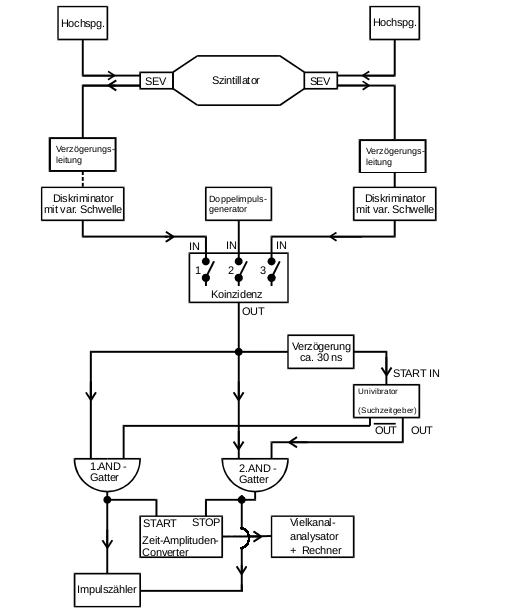
\includegraphics[width=0.7\linewidth,height=0.8\textheight,keepaspectratio]{Bilder/blockAdaptiert.png}
	\caption{Blockschaltbild der Messapparatur adaptiert \cite{Anl}}
	\label{FIG:Aufbau}
\end{figure}

\subsection{Justage}
Da die beiden SEVs unterschiedliche elektrische Eigenschaften besitzen, werden zunächst Verzögerungsleitungen einjustiert, sodass die Ausgangsrate nach der Koinzidenzschaltung maximal ist. Anschließend werden die Schwellwerte der Diskriminatoren einjustiert und die Suchzeit über den Univibrator eingestellt. Danach wird eine Kalbibration der Zeitachse vorgenommen und die Messung begonnen.

\section{Auswertung}

\subsection{Verzögerungsleitung}
Zunächst muss die Verzögerungsleitung so eingestellt werden, dass Signale, die von beiden SEVs gemessen wurden, auch nahezu gleichzeitig in der Koinzidenzschaltung ankommen. Es wird dazu die Verzögerung im ns Bereich variiert und die Zählrate direkt nach der Koinzidenzschaltung grafisch dargestellt. Die optimale Verzögerung liegt im Maximum der Zählrate.
Für alle folgenden Messungen wurde eine Verzögerung von -4\,\si{ns} empirisch gewählt, da die Messwerte in Tabelle \ref{tab:koinzidenz} kein eindeutiges Maximum aufweisen. Durch die folgende Rechnung soll gezeigt werden, dass diese Wahl zulässig war. 

\begin{figure}[htbp]
	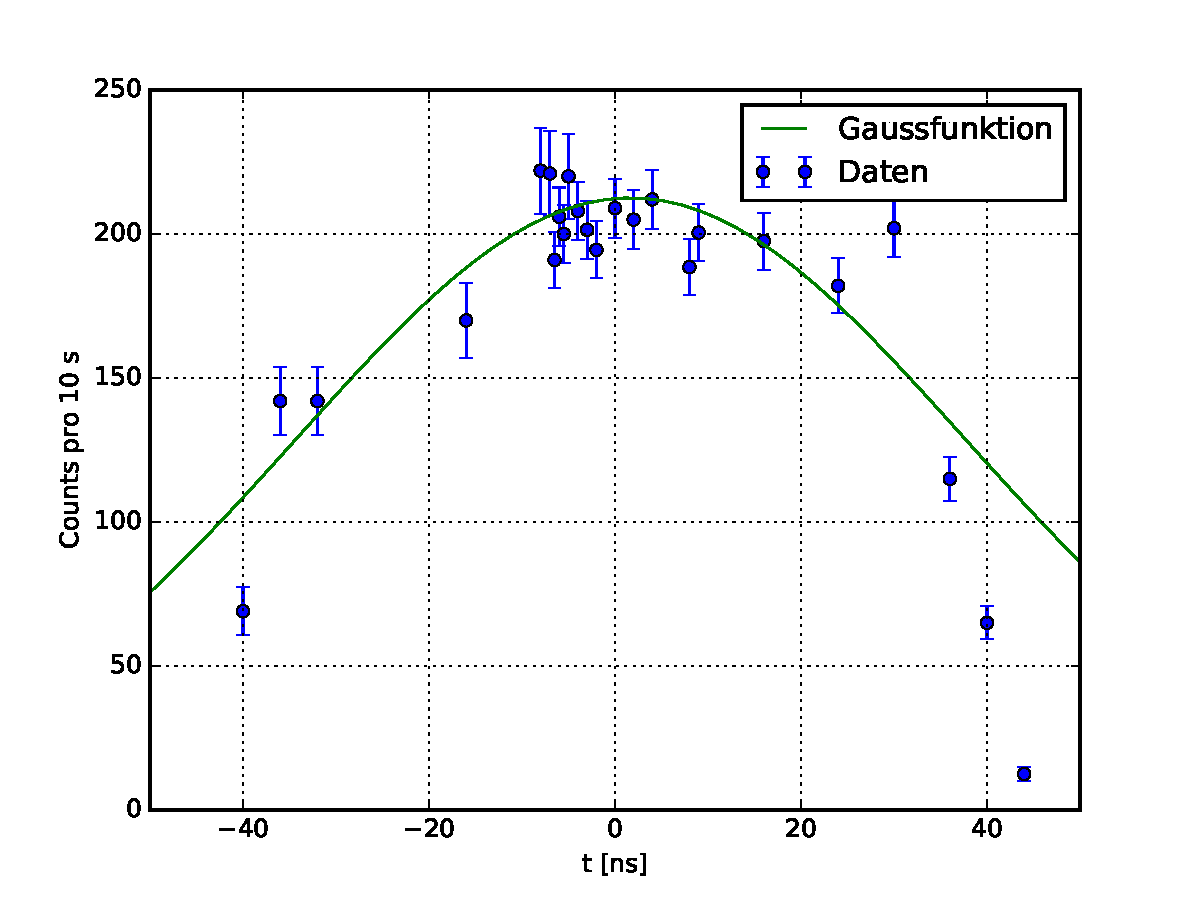
\includegraphics[width=0.8\textwidth]{./Bilder/koinzidenz.pdf}
	\caption{Zählrate gegen die zeitliche Verzögerung der Signale aufgetragen. Die Position des Maximums wird durch den Fit einer Gaussfunktion approximiert, um eine Abschätzung der Breite zu erhalten.}
	\label{fig:koinzidenz}
\end{figure}

\begin{table}[htbp]
	\input{../auswertung/Koinzidenz.dat}
	\caption{Messwerte für die Kalibrierung der Koinzidenzschaltung. t entspricht der relativen Verzögerung der Signale aus dem linken SEV gegenüber dem rechten.}
	\label{tab:koinzidenz}
\end{table}

Die gemessene Verteilung ist in Abbildung \ref{fig:koinzidenz} dargestellt und die Messwerte stehen in Tabelle \ref{tab:koinzidenz}. Der Fit einer Gausschen Normalverteilung
\begin{align}
	f(x,\mu,\sigma) = A\cdot e^{-\frac{(x-\mu)^2}{\sigma^2}}
\end{align}
wurde mit dem Python Paket scipy.optimize nach der Methode der kleinsten Quadrate durchgeführt, um eine Abschätzung über die Breite der Verteilung zu erhalten. Die Messwerte wurden mit dem Kehrwert der Standardabweichung gewichtet.
\begin{align}
A &= (231,89 \pm 6,42)\,\text{Counts}\\
\mu &= (-3,46 \pm 1,42)\,\si{ns}\\
\sigma &= ({26,56} \pm 3,53)\,\si{ns}
\end{align}
Die gefittete Gaussverteilung hat eine Standardabweichung von $\sigma = ({26,56} \pm 3,53)\,\si{ns}$ um den Mittelwert $\mu = (-3,46 \pm 1,42)\,\si{ns}$ herum. Daher ist die gewählte Verzögerung von \SI{-4}{ns} zulässig und sollte die folgenden Messungen nicht beeinflussen.

Nun werden die Thresholds der beiden Diskriminatoren nacheinander so eingestellt, dass die Zählrate der Startsignale jeweils bei etwa 22 Counts/s liegt. Dies entspricht in etwa der theoretisch erwarteten Zählrate von kosmischen Myonen bezogen auf die Fläche des Detektortankes \cite{Anl}. Durch die Thresholds soll möglichst der gesamte Untergrund, den die beiden Photomultiplyer durch thermisches Rauschen erzeugen, weggefiltert werden. Der Bruchteil des thermischen Rauschens, der dennoch den Threshold überschreitet, wird anschließend fast vollständig von der Koinzidenzschaltung weggefiltert. Dies wurde am Ende von Kap. \ref{kap:aufbau} beschrieben.

\subsection{Kalibrierung des Vielkanal-Analysators}
Der Zeit-Amplituden-Konverter wandelt die Zeitdifferenz zwischen dem Start- und dem Stoppsignal in eine Spannung um, die vom Vielkanalanalysator ausgelesen wird. Um den Zusammenhang zwischen Zeitdifferenz und Kanal zu erhalten, wird die Schaltung mit einem Doppelimpulsgenerator betrieben, der Signalpulse mit fest definiertem Abstand zueinander ausgibt. Es ist dadurch möglich, eine Korrelation zwischen dem zeitlichen Abstand zwischen den Pulsen und dem Kanal, dem dieses Signal zugeordnet wird zu finden. Wenn eine Zeitdifferenz auf mehrere direkt nebeneinander liegende Kanäle abgebildet wurde, so wurde als Kanal der gewichtete Mittelwert gewählt. Die Zeitdifferenz wird in 1\,\si{ns} Schritten von 1\,ns bis 9\,ns variiert und gegen die Channel ID in \mbox{Abbildung \ref{fig:linFit}} aufgetragen. Die Messwerte stehen in Tabelle \ref{tab:linFit}.

\begin{figure}[H]
	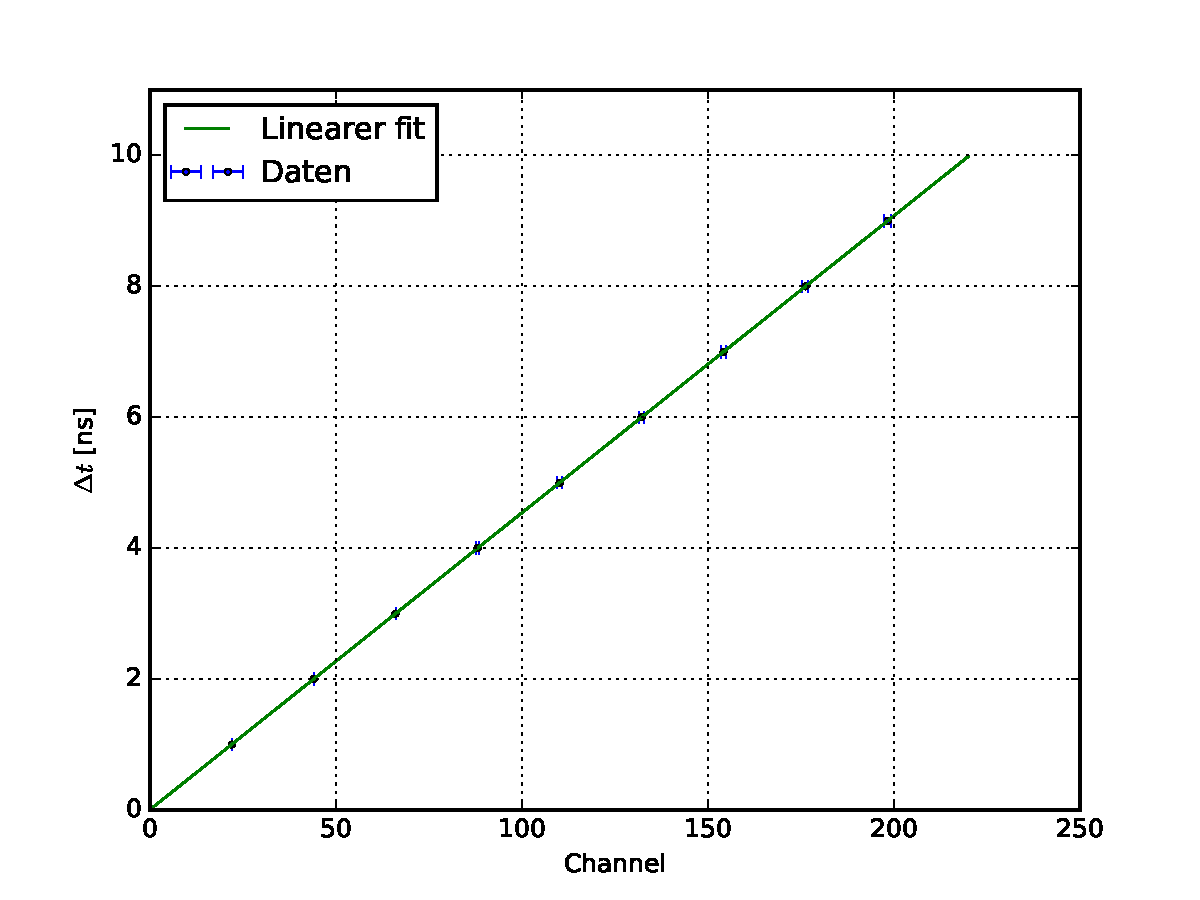
\includegraphics[width=0.8\textwidth]{./Bilder/linFit.pdf}
	\caption{Zeitdifferenz aus dem Doppelpulsgenerator gegen die Channel ID des Vielkanal-Analysators aufgetragen. Der Verlauf entspricht dem einer Geraden und die Fehlerbalken sind kleiner als die Datenpunkte.}
	\label{fig:linFit}
\end{figure}

\begin{table}[htbp]
	\input{../auswertung/LinFit.dat}
	\caption{Messwerte aus der Kalibrierung des Vielkanal-Analysators. Channel mit Nachkommastellen treten auf, wenn eine Messreihe auf mehrere benachbarte Channel abgebildet wurde. In diesem Fall wurde der gewichtete Mittelwert gebildet.}
	\label{tab:linFit}
\end{table}

Als Fitfunktion wurde eine Gerade der Form
\begin{align}
	f(x) = mx + b
	\label{eq:vielkanal}
\end{align}
verwendet. Der Fit ergab folgende Werte für die Parameter:
\begin{align}
	m &= (4,52 \pm 0,01) \cdot10^{-2} \,\frac{\si{ns}}{\text{Channel}}\\ 
	b &= (3,4 \pm 0,1) \cdot 10^{-3}\, \si{ns}
\end{align}

Da der Verlauf der Kurve für die ersten 200 Kanäle linear ist und nur sehr kleine Fehler aufweist, wird der Fit verwendet um alle 512 Kanäle auf Zeitintervalle abzubilden. Zudem werden für die weitere Rechnung die Fehler der Kalibrierung vernachlässigt, da diese sehr klein sind.

\subsection{Berechnung der Langzeit-Untergrundrate}
Während der Messung wurden $7894976$ Startsignale $N_\text{Start}$ in $t = \SI{246420}{s}$ detektiert. Dies entspricht einer mittleren Rate von 
\begin{align}
	\overline{N} = \frac{N_\text{Start}}{t} = 32,04\pm 0,01
\end{align}
Myonen pro Sekunde und liegt damit leicht oberhalb der erwarteten Rate von etwa 25 Myonen pro Sekunde \cite{Anl}. Die Diskriminatoren sind daher etwas zu niedrig eingestellt und lassen ein paar Untergrundsignale der SEVs passieren.
 
Es ist möglich, dass während der Suchzeit $t_S \approx \SI{12,5}{\micro\second}$ ein zweites Myon in den Tank eintritt und dessen Startsignal als das Stoppsignal des ersten interpretiert wird. Dieser Untergrund kann durch eine Poissonverteilung abgeschätzt werden. Die Wahrscheinlichkeit, dass ein zweites Myon während der Suchzeit detektiert wird beträgt:
\begin{align}
 	P(n=1) &= \frac{\left(\overline{N}\cdot t_S\right)^n}{n!}{e^{-\overline{N}\cdot t_S}} = (4,803 \pm 0,002)\cdot10^{-4}\\
 	\intertext{Somit wurden im Mittel}
 	N_b &= P(n=1)\cdot N_\text{Start} = 3792,35 \pm 2,70 
\end{align}
Hintergrundereignisse detektiert. Diese sind gleichförmig auf die Channel mit \mbox{$\Delta t < \SI{12,5}{\micro s}$} verteilt, da die endliche Suchzeit Einträge in höheren Channeln verhindert. Mit den Ergebnissen aus dem linearen Fit in Abbildung \ref{fig:linFit} ergibt sich für die Channelobergrenze:
\begin{align}
	\text{Channel}_\text{max} = \SI{12,5}{\micro s}\cdot\frac{1}{m} - \frac{b}{m} = 276,22 \pm 0,01\
\end{align}
Somit müssen pro Channel
\begin{align}
	U_\text{theo} = \frac{N_b}{\text{Channel}_\text{max}} = 13,73 \pm 0,01
	\label{untergrund}
\end{align}
Untergrundereignisse erwartet werden.
 

\subsection{Die Lebensdauer von Myonen}
Entsprechend des ermittelten linearen Zusammenhanges zwischen Kanal und Zeitdifferenz, kann nun für die durchgeführte Messung die Aufenthaltsdauer der Myonen im Detektortank in Abbildung \ref{fig:lebensdauer} visualisiert werden.
\begin{figure}[htb]
	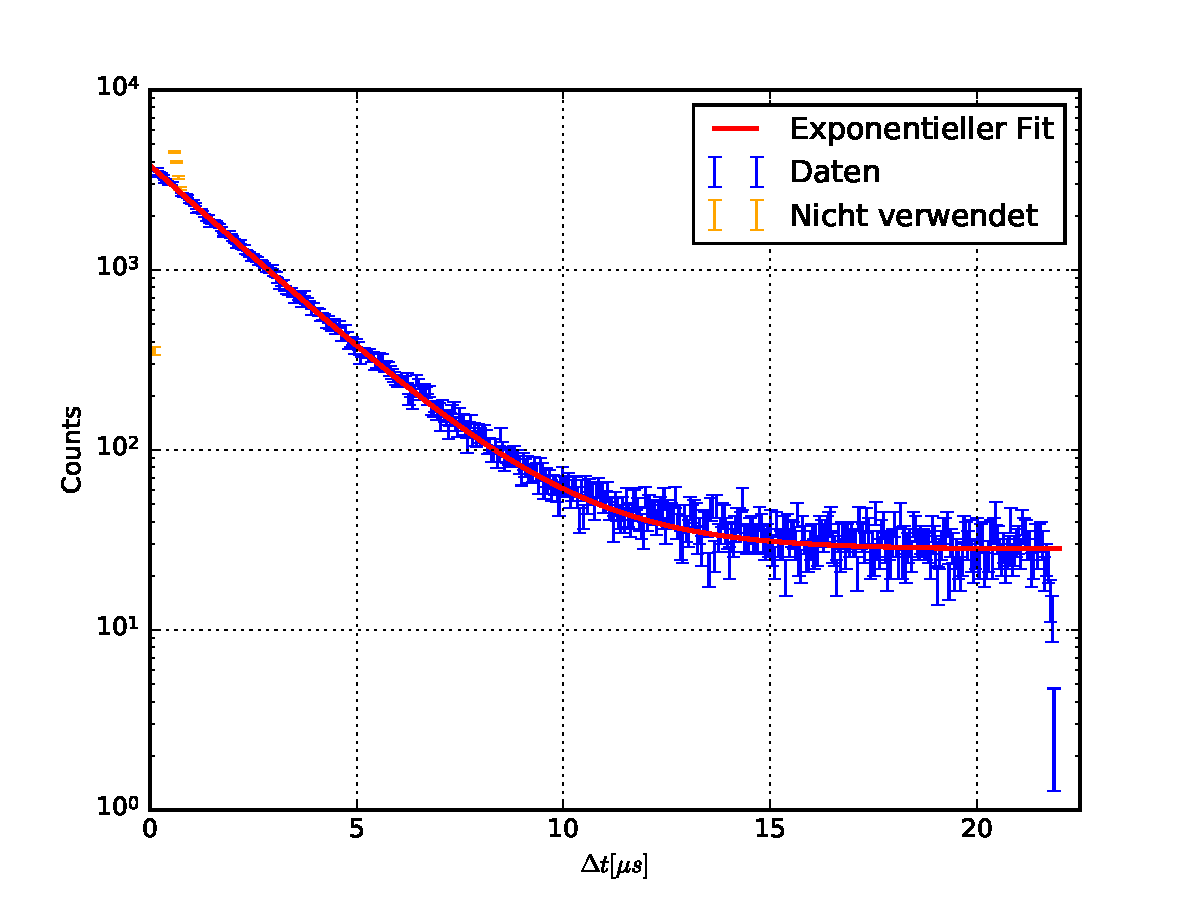
\includegraphics[width=0.8\textwidth]{./Bilder/lebensdauer_fit.pdf}
	\caption{Messwerte der kosmischen Myonen und an die Messwerte gefittete Exponentialfunktion.
	Die ersten drei Channel sowie Channel 14, 15, 16 und 17 wurden nicht verwendet, da die Werte zu stark nach unten bzw. nach oben abweichen. Eine genauere Diskussion der Bedeutung dieser Ausreißer erfolgt in Kap. \ref{kap:diskussion}. Auch Bins mit $\Delta t > \SI{12,5}{\micro s}$ wurden ignoriert, da die Verteilung aufgrund der endlichen Suchzeit hier abbricht.}
	\label{fig:lebensdauer}
\end{figure}
Als Verteilung wurde die Exponentialverteilung 
\begin{align}
	f(t) = N_0\cdot e^{-\lambda t} + U_\text{fit}
	\label{eq:zerfall}
\end{align}
zugrunde gelegt. Der Fit in Abbildung \ref{fig:lebensdauer} ergab für die mittlere Lebenszeit
\begin{align}
	\tau &= (2,11 \pm 0,02)\,\si{\micro\second}
\intertext{und für den konstanten Untergrund}
U_\text{fit} &= (4,78 \pm 1,08)\,\text{Counts}
\end{align}

\section{Diskussion}
\label{kap:diskussion}
Es gelang mit der Apparatur den Zerfall von Myonen im Detektortank nachzuweisen. Die berechnete mittlere Lebensdauer von $(2,11 \pm 0,02)\,\si{\micro\second}$ weicht um etwa 5\% vom Literaturwert\,\cite{PDG} mit 2,2\,\si{\micro\second} nach unten ab. Diese Abweichung kann dadurch erklärt werden, dass die Myonen mit den Atomen im Szintilatormedium wechselwirken und daher ihre Lebensdauer im Vergleich zu Myonen im Vakuum reduziert wird.

Die Berechnung des Untergrundes liefert leicht widersprüchliche Zahlenwerte von\\ \mbox{$13,73 \pm 0,01$ Counts} und $4,78\,\pm\,1,08\,\text{Counts}$. Dieser Unterschied entsteht durch den Peak in Abbildung \ref{fig:lebensdauer} bei etwa 0,7\,\si{\micro s}. Die Ausreißer wurden nicht für den Fit verwendet, sie beeinflussen jedoch den theoretischen Untergrund (vgl. Gleichung(\ref{untergrund})), da es zusätzliche Startsignale sind. Ursache für den Peak könnte ein Fehler in der Verkabelung sein, durch den Reflektionen falsche Signale erzeugen.

Der Vielkanalanalysator hat insgesamt 36908 Stoppsignale detektiert, es fehlen damit 3361 im Vergleich zu der Anzahl, die der Impulszähler gezählt hat. An dem Inhalt der Histogrammbins wird ersichtlich, dass in den ersten zwei Bins garkeine und im dritten nur 94 Signale enthalten sind. Bei einer Erwartung von durchschnittlich 700 Signalen pro Bin entspricht dies insgesamt 2006 fehlenden Signalen. Es scheint daher, dass der Zeit-Amplituden-Converter oder der Vielkanalanalysator diese besonders kurzen Signale nicht detektieren kann und vielleicht auch in den nächst höheren Bins noch weniger sensitiv als in den Übrigen ist.

Insgesamt wurden im Zeitraum der Messung 7894976 Startsignale detektiert, von denen jedoch nur 40269 innerhalb der vorgegebenen Suchzeit von etwa $\SI{12,5}{\micro\second}$ ein Stoppsignal erhalten haben. Es sind somit nur etwa 0,51\% der einfallenden kosmischen Myonen im Detektor vollkommen abgebremst und zerfallen. Daher ist es notwendig, die Messung über einen Zeitraum von mehreren Tagen durchzuführen um genug Statistik zu erhalten.

%\clearpage
\vfill
\begin{thebibliography}{WissOnl}
\bibitem{Anl} TU Dortmund Versuchsanleitung zu Versuch Nr.01 (abgerufen am 20.6.2014) \url{http://129.217.224.2/HOMEPAGE/PHYSIKER/BACHELOR/FP/SKRIPT/V01.pdf}

\bibitem{PDG} Particle Data Group. Particle physics booklet. Institute of Physics publishing, 2006.

\end{thebibliography}
\end{document}
